% Provenance (never printed): old terminale S material on mountain ranges and
% continental collision (folds, reverse faults and nappes as signs of
% shortening and thickening; ophiolites and sutures as the trace of a closed
% ocean; the Himalaya and the Alps as examples). Owner (Sync 0): collision,
% fold/anticline/syncline/fold axis, reverse fault/thrust, nappe, ophiolite,
% suture, shortening. Fault is Book 1's (g7), normal fault g11.05's, the root
% and Airy isostasy g11.03's and g12.01's: recalled, never redefined. India's
% past latitudes: figdata/grade-12/india_drift.py (GPlates Web Service, two
% published plate models); shortening: figdata/grade-12/fold_shortening.py;
% the belt map: figdata/grade-12/alpine_belt.py.
\chapter{造山运动}\label{ch:g12:mountain-building}

登上珠穆朗玛峰的攀登者，所处之地高出海平面 \qty{8848.86}{m}，
脚下踩的是石灰岩。从峰顶带回样品的地质学家
在其中发现了三叶虫、介形虫和
海百合的碎片：这些海洋生物距今超过 44000 万年，生活于
奥陶纪。世界上最高的岩石，沉积于一片
海底。本章解释海底如何登上“世界屋脊”：
两大陆相撞，二者之间的地壳被挤压、\omterm{def:g12:mountain-building:fold}{褶皱}、
叠置并增厚，形成山脉。
% ledger: sakai05:summit, tulane:roots (marine limestones at the top of Mt. Everest), ics:base.Ordovician, ics:base.Silurian (486.85-443.1 Ma); Book 1: tht:everest (8848.86 m)

\begin{omfigure}
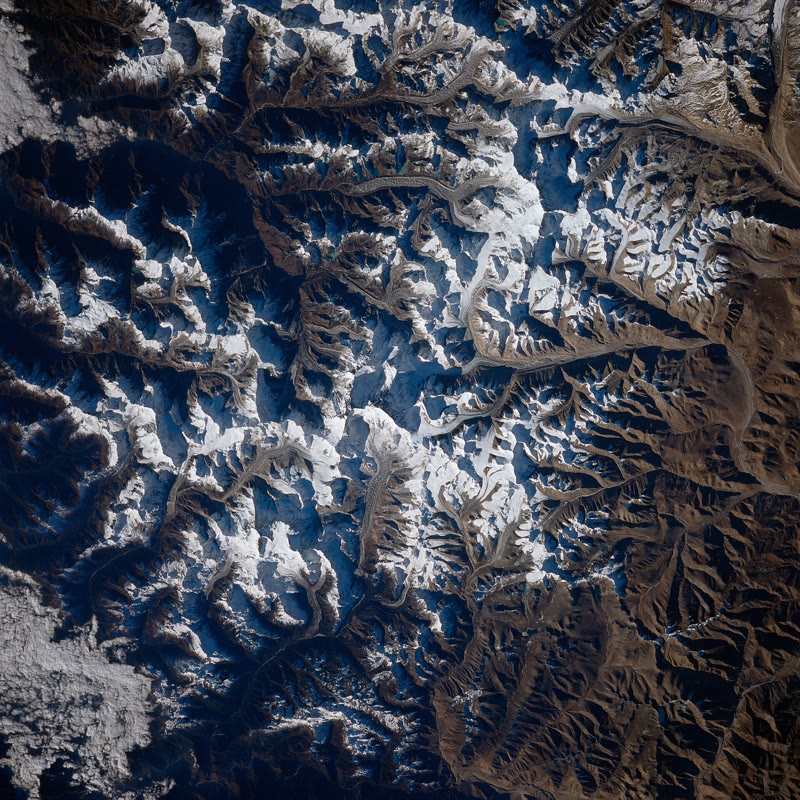
\includegraphics[width=0.5\linewidth]{images/book2/g12-nasa-everest-columbia.jpg}

{\small 从哥伦比亚号航天飞机上所见的珠穆朗玛峰及周围众多冰川，1996 年 11 月 30 日拍摄。
照片：NASA（公有领域）。}
\end{omfigure}
% ledger: photo:g12-everest-columbia

\begin{recall}
在洋脊处生成的\omterm{def:g11:ocean-ridges:oceanic-lithosphere}{大洋岩石圈}板块，
于海沟处沉回地幔；其\omterm{def:g11:subduction-zones:slab-pull}{板片拉力}将其拉下（见\cref{ch:g11:subduction-zones}）。
陆壳厚而轻，平均密度约为 \qty{2830}{kg/m^3}，
其下地幔的密度为 \qty{3380}{kg/m^3}，陆壳因而漂浮得较高，且
厚壳比薄壳站得更高，其下有
地壳根（见\cref{ch:g12:continental-crust,ch:g11:lithosphere-asthenosphere}）。
断层是两侧岩块发生相对位移的破裂面；在\omterm{def:g11:ocean-ridges:normal-fault}{正断层}处，
断层面以上的岩块下降，
如地壳在慢速洋脊处被拉张时那样（见\cref{ch:g11:ocean-ridges}）。
\end{recall}
% ledger: cm95:crust, data:prem, tulane:no-subduct, usgs:normal-fault

\section{从俯冲到碰撞}

若大洋在海沟处的消亡速度快于其在洋脊处的生成速度，
大洋便会缩小。骑在下沉板块上的大陆
以板块的速度靠近海沟，最终抵达海沟。
\omterm{def:g11:ocean-ridges:oceanic-lithosphere}{大洋岩石圈}已在其前方下沉；大陆无法随之
下沉，因其地壳太轻，不能沉入密度更大的地幔。\omterm{def:g11:subduction-zones:subduction}{俯冲}
停止。两大陆相互挤压，而
自洋底垂下的\omterm{def:g11:subduction-zones:slab}{板片}最终断裂，
沉入地幔。
% ledger: earle:collision, tulane:no-subduct

\begin{definition}[大陆碰撞]\label{def:g12:mountain-building:collision}
称\emph{大陆碰撞}\index{大陆碰撞}为
两大陆在汇聚板块边界处相遇，且二者之间的
\omterm{def:g11:ocean-ridges:oceanic-lithosphere}{大洋岩石圈}已被\omterm{def:g11:subduction-zones:subduction}{俯冲}消减。两大陆均不下沉，二者之间的地壳
发生变形并增厚，形成造山带。
\end{definition}
% ledger: earle:collision, tulane:no-subduct, usgs:himalaya-collision

\begin{omfigure}
\begin{tikzpicture}[x=0.95cm, y=0.95cm, font=\scriptsize]
  % ---- stage 1: the ocean closes ----
  \begin{scope}[yshift=0cm]
    \fill[omSea] (3.4,0) -- (8.6,0) -- (8.0,-0.5) -- (4.3,-0.5) -- (3.5,0.0) -- cycle;
    \fill[omLithGranite] (0,0.15) -- (3.5,0.15) -- (4.3,-0.5) -- (4.3,-0.75) -- (3.5,-1.0) -- (0,-1.0) -- cycle;
    \fill[omLithBasalt] (4.3,-0.5) -- (8.0,-0.5) .. controls (9.0,-0.75) and (9.6,-1.2) .. (10.4,-2.0)
      -- (10.15,-2.15) .. controls (9.4,-1.4) and (8.9,-1.0) .. (8.0,-0.75) -- (4.3,-0.75) -- cycle;
    \fill[omLithGranite] (8.0,-0.5) -- (8.6,0.2) -- (12,0.2) -- (12,-1.05) -- (9.5,-1.05)
      .. controls (9.0,-0.75) .. (8.0,-0.5) -- cycle;
    \fill[omThm!70] (10.0,0.2) -- (10.3,0.55) -- (10.6,0.2) -- cycle;
    \draw[black!60, line width=0.3pt] (0,0.15) -- (3.5,0.15) -- (4.3,-0.5) -- (8.0,-0.5) -- (8.6,0.2) -- (12,0.2);
    \draw[-{Stealth[length=2mm]}, line width=0.8pt] (1.2,0.45) -- (2.6,0.45);
    \node[anchor=east] at (0,-0.4) {1};
    \node at (1.8,-0.5) {大陆};
    \node at (6.1,-0.25) {海洋};
    \node[anchor=north] at (6.1,-0.8) {大洋岩石圈};
    \node[anchor=south] at (8.0,0.0) {海沟};
    \node[anchor=south] at (10.3,0.55) {火山弧};
    \node at (11.1,-0.5) {大陆};
  \end{scope}
  % ---- stage 2: the continents meet ----
  \begin{scope}[yshift=-3.0cm]
    \fill[omSea] (6.9,0) -- (8.4,0) -- (8.0,-0.4) -- (7.4,-0.35) -- cycle;
    \fill[omLithGranite] (0,0.15) -- (6.8,0.15) -- (7.6,-0.4) -- (8.0,-0.5)
      .. controls (9.0,-0.75) .. (9.5,-1.05) -- (9.2,-1.4) -- (6.5,-1.0) -- (0,-1.0) -- cycle;
    \fill[omLithBasalt] (9.5,-1.05) .. controls (10.0,-1.4) .. (10.6,-2.0) -- (10.35,-2.15)
      .. controls (9.8,-1.6) .. (9.2,-1.4) -- cycle;
    \fill[omLithGranite] (8.0,-0.5) -- (8.6,0.2) -- (12,0.2) -- (12,-1.05) -- (9.5,-1.05)
      .. controls (9.0,-0.75) .. (8.0,-0.5) -- cycle;
    \fill[omLithPeridotite] (7.0,0.15) -- (7.9,0.15) -- (8.3,0.05) -- (7.95,-0.12) -- (7.3,0.0) -- cycle;
    \fill[omThm!70] (10.0,0.2) -- (10.3,0.55) -- (10.6,0.2) -- cycle;
    \draw[-{Stealth[length=2mm]}, line width=0.8pt] (3.2,0.45) -- (4.6,0.45);
    \node[anchor=east] at (0,-0.4) {2};
    \node at (3.4,-0.45) {大陆};
    \draw[black!60] (7.6,0.12) -- (7.0,0.75) node[anchor=south east, inner sep=1pt] {洋底切片};
    \node at (11.1,-0.5) {大陆};
    \node[anchor=west] at (10.7,-1.9) {板片};
  \end{scope}
  % ---- stage 3: a mountain belt ----
  \begin{scope}[yshift=-6.4cm]
    \fill[omLithGranite] (0,0.15) -- (4.5,0.15) .. controls (6.0,0.4) and (6.6,1.25) .. (7.6,1.3)
      .. controls (8.7,1.3) and (9.6,0.5) .. (10.6,0.2) -- (12,0.2) -- (12,-1.05) -- (10.6,-1.1)
      .. controls (9.5,-2.2) and (8.6,-2.6) .. (7.7,-2.6) .. controls (6.6,-2.6) and (5.6,-1.6) .. (4.5,-1.0)
      -- (0,-1.0) -- cycle;
    \draw[black!60, line width=0.3pt] (0,0.15) -- (4.5,0.15) .. controls (6.0,0.4) and (6.6,1.25) .. (7.6,1.3)
      .. controls (8.7,1.3) and (9.6,0.5) .. (10.6,0.2) -- (12,0.2);
    \draw[black!60, dashed, line width=0.4pt] (0,-1.0) -- (4.5,-1.0) .. controls (5.6,-1.6) and (6.6,-2.6) .. (7.7,-2.6)
      .. controls (8.6,-2.6) and (9.5,-2.2) .. (10.6,-1.1) -- (12,-1.05);
    \draw[omThm, line width=1.0pt] (7.0,1.25) -- (8.3,-2.55);
    \foreach \t in {0.15,0.4,0.65}
      \fill[omLithPeridotite] ($(7.0,1.25)!\t!(8.3,-2.55)$) ++(-0.12,0.05) -- ++(0.3,0) -- ++(-0.05,-0.22) -- ++(-0.3,0) -- cycle;
    \fill[omLithBasalt] (10.9,-1.9) -- (11.5,-2.35) -- (11.35,-2.5) -- (10.75,-2.05) -- cycle;
    \node[anchor=east] at (0,-0.4) {3};
    \node at (2.4,-0.45) {大陆};
    \node at (11.3,-0.5) {大陆};
    \draw[black!60] (7.2,0.6) -- (5.9,1.5) node[anchor=east, inner sep=1pt] {缝合带与蛇绿岩};
    \node at (7.7,-1.9) {地壳根};
    \node[anchor=north] at (11.2,-2.5) {断离板片};
    \node[anchor=south] at (7.6,1.35) {造山带};
  \end{scope}
\end{tikzpicture}

{\small 从\omterm{def:g11:subduction-zones:subduction}{俯冲}到碰撞（未按比例）。1：洋盆闭合，
其洋底在海沟处下沉。2：大陆抵达海沟，
无法下沉，洋底的碎片被推挤到其边缘。3：两大陆之间的地壳
被缩短、加厚，形成位于一个根部之上的造山带；
两大陆相接处的线，由洋底碎片标示，
即为\omterm{def:g12:mountain-building:suture}{缝合带}；\omterm{def:g11:subduction-zones:slab}{板片}断离并下沉。}
\end{omfigure}
% ledger: earle:collision, tulane:ocean-basins, usgs:suture, tulane:roots

\subsection{消失洋盆的遗迹}

洋盆闭合后，两大陆沿一条线焊接在一起。

\begin{definition}[缝合带]\label{def:g12:mountain-building:suture}
称\emph{缝合带}\index{缝合带}为两大陆之间的线或狭窄带，两大陆
经碰撞而相接，且二者之间的\omterm{def:g11:subduction-zones:subduction}{俯冲}已经停止：
它是古板块边界的遗迹，标示出两者之间
洋盆曾经所在的位置。
\end{definition}
% ledger: usgs:suture, liu20:itsz

什么标志着\omterm{def:g12:mountain-building:suture}{缝合带}？沿许多\omterm{def:g12:mountain-building:suture}{缝合带}分布的岩体，
在大陆上并不常见：自上而下依次为海相沉积物、枕状玄武岩、
一套并排直立的\omterm{def:g11:igneous-rocks:intrusion}{岩墙}、\omterm{def:g11:ocean-ridges:gabbro}{辉长岩}，以及位于底部的
地幔\omterm{def:g11:ocean-ridges:peridotite}{橄榄岩}：此即洋底的层序
（见\cref{ch:g11:ocean-ridges}），其下为地幔顶部。
% ledger: tulane:ocean-basins

\begin{definition}[蛇绿岩]\label{def:g12:mountain-building:ophiolite}
称\emph{蛇绿岩}\index{蛇绿岩}为一块\omterm{def:g11:ocean-ridges:oceanic-lithosphere}{大洋岩石圈}——
由沉积物、枕状玄武岩、席状\omterm{def:g11:igneous-rocks:intrusion}{岩墙}、\omterm{def:g11:ocean-ridges:gabbro}{辉长岩}和地幔\omterm{def:g11:ocean-ridges:peridotite}{橄榄岩}组成——
被推覆到\omterm{def:g12:continental-crust:continental-crust}{大陆地壳}之上。
\end{definition}
% ledger: tulane:ocean-basins

\omterm{def:g12:mountain-building:ophiolite}{蛇绿岩}是搁浅的洋底：消失洋盆的一块碎片，被推覆
到大陆上，而未随其余部分一同下沉。碰撞抬升的山脉
通常包含部分\omterm{def:g11:ocean-ridges:oceanic-lithosphere}{洋壳}和上地幔，因为洋盆正是在此闭合。
在藏南，沿印度河–雅鲁藏布\omterm{def:g12:mountain-building:suture}{缝合带}
分布的\omterm{def:g12:mountain-building:ophiolite}{蛇绿岩}是名为新特提斯洋的古洋残余，
该洋位于印度与拉萨地区之间；在此处，一块\omterm{def:g11:ocean-ridges:gabbro}{辉长岩}
的年龄被测定为 2.43 亿年。
% ledger: tulane:ocean-basins, earle:collision, liu20:itsz

\begin{omfigure}
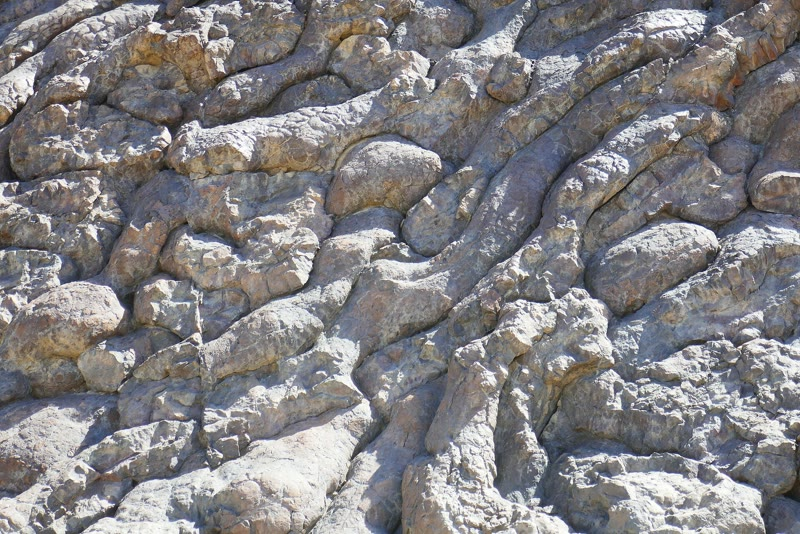
\includegraphics[width=0.6\linewidth]{images/book2/g12-duchoiselle-oman-pillows.jpg}

{\small 阿曼吉兹谷（Wadi Jizzi）的塞迈勒\omterm{def:g12:mountain-building:ophiolite}{蛇绿岩}枕状熔岩：熔岩曾在水下冷却，
如今已位于陆地上。照片：Lionel
Duchoiselle（CC~BY-SA~3.0）。}
\end{omfigure}
% ledger: photo:g12-oman-pillows

\section{地壳的缩短}

岩体受侧向挤压时，若处于低温且脆性，则会断裂；若
温度足够高而表现为塑性，则会发生\omterm{def:g12:mountain-building:fold}{褶皱}。造山带
中既有\omterm{def:g12:mountain-building:fold}{褶皱}，也有断层。
% ledger: earle:folds

\subsection{褶皱}

\begin{definition}[褶皱；背斜；向斜；褶皱轴]\label{def:g12:mountain-building:fold}
称\emph{褶皱}\index{褶皱}为岩层的弯曲。其倾斜的两翼
称为\emph{翼}；两翼相交于\emph{转折端}，
即岩层弯曲最甚处，沿转折端的线即为
\emph{褶皱轴}\index{褶皱轴}。\emph{背斜}\index{背斜}是岩层向上弯曲的褶皱，
其两翼远离轴线倾斜；
\emph{向斜}\index{向斜}是岩层向下弯曲的褶皱，其
两翼朝向轴线倾斜。
\end{definition}
% ledger: earle:folds, tulane:fold-geometry

各层转折端连成的平面即为轴面。
\omterm{def:g12:mountain-building:fold}{背斜}与\omterm{def:g12:mountain-building:fold}{向斜}通常成对出现，一者的翼
即为相邻一者的翼。\omterm{def:g12:mountain-building:fold}{褶皱}大小不一，从微观到数十
千米不等。经侵蚀后，\omterm{def:g12:mountain-building:fold}{背斜}的核部显示最老的岩层，\omterm{def:g12:mountain-building:fold}{向斜}
则显示最新的岩层；\omterm{def:g12:mountain-building:fold}{背斜}未必是山脊，
\omterm{def:g12:mountain-building:fold}{向斜}也未必是山谷，因侵蚀是沿软硬不同的岩层进行，
而非沿\omterm{def:g12:mountain-building:fold}{褶皱}的形状进行。
% ledger: earle:folds, tulane:fold-geometry

\begin{omfigure}
\begin{tikzpicture}[x=1.2cm, y=1.2cm, font=\scriptsize]
  \def\W{6}\def\H{2.0}\def\dx{1.35}\def\dy{0.78}
  \tikzset{declare function={zb(\x,\c)=\c+0.8*cos(60*(\x-1.5));}}
  \colorlet{bandA}{omLithSchist!70}\colorlet{bandB}{omLithSand}\colorlet{bandC}{omLithShale}
  \colorlet{bandD}{icsJurassic!35}\colorlet{bandE}{icsTriassic!35}\colorlet{bandF}{icsCretaceous!45}
  % front face
  \begin{scope}
    \clip (0,0) rectangle (\W,\H);
    \fill[bandA] (0,0) rectangle (\W,\H);
    \foreach \c/\col in {0.0/bandB, 0.6/bandC, 1.2/bandD, 1.8/bandE, 2.4/bandF}
      \fill[\col] plot[domain=0:\W, samples=80, smooth] (\x,{zb(\x,\c)}) -- (\W,4) -- (0,4) -- cycle;
    \foreach \c in {0.0,0.6,1.2,1.8,2.4}
      \draw[black!55, line width=0.35pt] plot[domain=0:\W, samples=80, smooth] (\x,{zb(\x,\c)});
  \end{scope}
  % top face: outcrop bands (crossings of the top surface computed for these curves)
  \fill[bandE] (0,\H) -- (0.242,\H) -- ++(\dx,\dy) -- (\dx,\H+\dy) -- cycle;
  \fill[bandD] (0.242,\H) -- (2.758,\H) -- ++(\dx,\dy) -- (0.242+\dx,\H+\dy) -- cycle;
  \fill[bandE] (2.758,\H) -- (3.5,\H) -- ++(\dx,\dy) -- (2.758+\dx,\H+\dy) -- cycle;
  \fill[bandF] (3.5,\H) -- (5.5,\H) -- ++(\dx,\dy) -- (3.5+\dx,\H+\dy) -- cycle;
  \fill[bandE] (5.5,\H) -- (\W,\H) -- ++(\dx,\dy) -- (5.5+\dx,\H+\dy) -- cycle;
  \foreach \x in {0.242,2.758,3.5,5.5} \draw[black!55, line width=0.35pt] (\x,\H) -- ++(\dx,\dy);
  % right face: the layers meet it at constant heights (cylindrical folds)
  \foreach \lo/\hi/\col in {0.0/0.6/bandB, 0.6/1.2/bandC, 1.2/1.8/bandD, 1.8/2.0/bandE}
    \fill[\col] (\W,\lo) -- (\W+\dx,\lo+\dy) -- (\W+\dx,\hi+\dy) -- (\W,\hi) -- cycle;
  \foreach \y in {0.6,1.2,1.8} \draw[black!55, line width=0.35pt] (\W,\y) -- ++(\dx,\dy);
  % outline
  \draw[black, line width=0.5pt] (0,0) rectangle (\W,\H) (0,\H) -- (\dx,\H+\dy) -- (\W+\dx,\H+\dy) -- (\W,\H)
    (\W+\dx,\H+\dy) -- (\W+\dx,\dy) -- (\W,0);
  % fold axes on the top face, axial planes on the front face
  \draw[omThm, line width=1pt] (1.5,\H) -- ++(\dx,\dy);
  \draw[omDef, line width=1pt] (4.5,\H) -- ++(\dx,\dy);
  \draw[omThm, dashed, line width=0.6pt] (1.5,0) -- (1.5,\H);
  \draw[omDef, dashed, line width=0.6pt] (4.5,0) -- (4.5,\H);
  \node[anchor=south, omThm] at (1.5+\dx,\H+\dy) {背斜：褶皱轴};
  \node[anchor=south, omDef] at (4.5+\dx,\H+\dy) {向斜：褶皱轴};
  \draw[black!70] (3.2,0.95) -- (3.9,-0.35) node[anchor=north] {翼};
  \draw[black!70] (1.5,1.4) circle (0.07) -- (0.4,-0.35) node[anchor=north] {转折端};
  \draw[black!70] (1.5,0.25) -- (2.0,-0.35) node[anchor=north] {轴面};
\end{tikzpicture}

{\small \omterm{def:g12:mountain-building:fold}{背斜}与\omterm{def:g12:mountain-building:fold}{向斜}被一个平坦的侵蚀面切开（块状示意图，未按比例绘制）。
\omterm{def:g12:mountain-building:fold}{褶皱轴}沿转折端延伸，虚线为轴面的迹线。
在顶面上，被侵蚀的\omterm{def:g12:mountain-building:fold}{背斜}核部显示较老的地层，
\omterm{def:g12:mountain-building:fold}{向斜}核部则显示较新的地层。}
\end{omfigure}
% ledger: earle:folds, tulane:fold-geometry

\begin{omfigure}
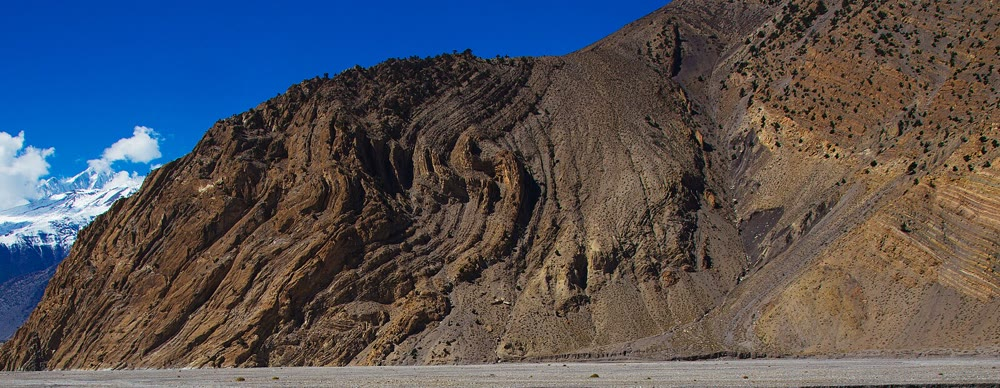
\includegraphics[width=0.95\linewidth]{images/book2/g12-hullot-kali-gandaki-folds.jpg}

{\small 喜马拉雅山一处悬崖中的\omterm{def:g12:mountain-building:fold}{褶皱}岩层，位于乔姆松东北约
\qty{3}{km}处的卡利甘达基峡谷，尼泊尔。
照片：Jean-Marie Hullot（CC~BY~2.0）。}
\end{omfigure}
% ledger: photo:g12-kali-gandaki

瓦尔登丘陵的\omterm{def:g11:fossil-fuel-geology:reservoir}{盖层}以同样的方式\omterm{def:g12:mountain-building:fold}{褶皱}，但要平缓得多。
其砂岩、石灰岩、页岩和白垩原本近水平沉积，
随后弯曲成一个\omterm{def:g12:mountain-building:fold}{背斜}和一个\omterm{def:g12:mountain-building:fold}{向斜}，两翼倾角为\ang{12}；
其后的一条\omterm{def:g11:ocean-ridges:normal-fault}{正断层}切穿了它们。
% ledger: region:name; model in figdata/shared/region.py (LIMB_DIP 12, AXIS_ANTI 3.5 km, AXIS_SYN 7.5 km)

\begin{omfigure}
\begin{tikzpicture}
\begin{axis}[omsection, x=1.25cm, y=0.003125cm, xmin=0, xmax=9.49, ymin=-700, ymax=650,
  xlabel={距 A 点的距离（\unit{km}）}, ylabel={高程（\unit{m}）},
  ytick={-600,-300,0,300,600}, tick label style={font=\scriptsize}]
\addplot[fill=black!8, draw=black!50, line width=0.3pt, even odd rule] table {figdata/out/shared-region-section-unit-schist.dat};
\addplot[fill=icsTriassic!20, draw=black!50, line width=0.3pt, even odd rule] table {figdata/out/shared-region-section-unit-sandstone.dat};
\addplot[fill=icsJurassic!25, draw=black!50, line width=0.3pt, even odd rule] table {figdata/out/shared-region-section-unit-limestone.dat};
\addplot[fill=icsJurassic!8, draw=black!50, line width=0.3pt, even odd rule] table {figdata/out/shared-region-section-unit-shale.dat};
\addplot[fill=icsCretaceous!20, draw=black!50, line width=0.3pt, even odd rule] table {figdata/out/shared-region-section-unit-chalk.dat};
\addplot[fill=omLithAlluv, draw=black!50, line width=0.3pt, even odd rule] table {figdata/out/shared-region-section-unit-alluvium.dat};
\addplot[black, line width=0.7pt] table {figdata/out/shared-region-section-ground.dat};
\addplot[fault] table {figdata/out/shared-region-section-fault.dat};
% axis positions from figdata/grade-12/fold_shortening.py (section_anticline_km, section_syncline_km; the syncline lies on the hanging wall, shifted by the fault heave)
\draw[omThm, dashed, line width=0.7pt] (axis cs:3.162,-700) -- (axis cs:3.162,660);
\draw[omDef, dashed, line width=0.7pt] (axis cs:7.484,-700) -- (axis cs:7.484,660);
\node[anchor=south, omThm, font=\scriptsize] at (axis cs:3.162,660) {背斜轴};
\node[anchor=south, omDef, font=\scriptsize] at (axis cs:7.484,660) {向斜轴};
\node[anchor=south east, font=\small\bfseries] at (axis cs:0,650) {A};
\node[anchor=south west, font=\small\bfseries] at (axis cs:9.49,650) {B};
\node[font=\scriptsize, fill=white, inner sep=1pt] at (axis cs:1.2,-520) {片岩};
\node[font=\scriptsize, fill=white, inner sep=1pt, anchor=east] at (axis cs:6.55,-450) {正断层};
\end{axis}
\end{tikzpicture}

\smallskip
{\small\tikz\fill[black!8, draw=black!50] (0,0) rectangle (0.35,0.22);~片岩 \quad
\tikz\fill[icsTriassic!20, draw=black!50] (0,0) rectangle (0.35,0.22);~砂岩 \quad
\tikz\fill[icsJurassic!25, draw=black!50] (0,0) rectangle (0.35,0.22);~石灰岩 \quad
\tikz\fill[icsJurassic!8, draw=black!50] (0,0) rectangle (0.35,0.22);~页岩 \quad
\tikz\fill[icsCretaceous!20, draw=black!50] (0,0) rectangle (0.35,0.22);~白垩 \quad
\omve{2.5}}

{\small 瓦尔登丘陵剖面 A--B，自西南向东北。\omterm{def:g11:fossil-fuel-geology:reservoir}{盖层}覆于
片岩基底之上，被\omterm{def:g12:mountain-building:fold}{褶皱}成一个\omterm{def:g12:mountain-building:fold}{背斜}和一个\omterm{def:g12:mountain-building:fold}{向斜}；
晚于\omterm{def:g12:mountain-building:fold}{褶皱}形成的\omterm{def:g11:ocean-ridges:normal-fault}{正断层}使东北侧断块下降。
垂直比例尺放大了 2.5 倍，这使
翼部看起来比实际更陡。数据取自本系列的
该区域模型。}
\end{omfigure}
% ledger: region:name; computed in figdata/shared/region.py (section A-B)

\subsection{逆断层、逆冲与推覆体}

地壳在冷而脆的状态下受挤压时，会沿断层破裂，
这类断层不同于拉张地壳中的\omterm{def:g11:ocean-ridges:normal-fault}{正断层}。

\begin{definition}[逆断层；逆冲]\label{def:g12:mountain-building:thrust}
称\emph{逆断层}\index{逆断层}为一种倾斜断层，沿该断层，
断层面上方的断块相对于下方的断块向上运动。
逆断层形成于地壳受挤压之处。称
\emph{逆冲}\index{逆冲}是倾角较缓的逆断层，倾角小于
\ang{45}。
\end{definition}
% ledger: earle:reverse-thrust, tulane:fold-geometry

\omterm{def:g12:mountain-building:thrust}{逆冲}可将一层岩石推移数十千米，使较老的岩层
覆于较新岩层之上，与岩层原有的沉积顺序相反。
在落基山脉，麦康内尔\omterm{def:g12:mountain-building:thrust}{逆冲}断层
已将一套厚约\qty{800}{m}的沉积岩系自西向东推移约\qty{40}{km}：
现今，约 5 亿年的石灰岩覆于
约 7500 万年的泥岩之上。
% ledger: earle:reverse-thrust

\begin{definition}[推覆体]\label{def:g12:mountain-building:nappe}
称\emph{推覆体}\index{推覆体}为一大片岩石，它
被搬运了很长距离（常达数十千米），越过其下的岩石，
沿一条近于水平的\omterm{def:g12:mountain-building:thrust}{逆冲}断层移动。
\end{definition}
% ledger: ngu:nappe, earle:reverse-thrust

\omterm{def:g12:mountain-building:nappe}{推覆体}可搬运远处形成的岩石，甚至包括洋底的\omterm{def:g11:minerals:thin-section}{薄片}；它
自身也可能被\omterm{def:g12:mountain-building:fold}{褶皱}，岩层可能倒转。造山带中\omterm{def:g12:mountain-building:nappe}{推覆体}
一层压着一层地叠置。后期侵蚀会切穿\omterm{def:g12:mountain-building:nappe}{推覆体}，开出
通向下伏岩石的“窗”，并留下孤立的残块，
立于较新的岩层之上。
% ledger: ngu:nappe

\begin{omfigure}
\begin{tikzpicture}[x=1.0cm, y=1.0cm, font=\scriptsize]
  % rocks in place (younger), flat-lying
  \fill[icsCretaceous!25] (0,-1.6) rectangle (12,-0.4);
  \fill[icsJurassic!25] (0,-1.6) rectangle (12,-1.1);
  \draw[black!50, line width=0.3pt] (0,-1.1) -- (12,-1.1);
  \fill[white] (5.6,-0.4) -- (6.2,-0.62) -- (6.8,-0.4) -- cycle;
  % the nappe (older rocks) above a nearly flat thrust, cut by erosion
  \fill[omLithSchist!80] (0.8,-0.4) .. controls (1.2,0.35) and (1.9,0.35) .. (2.3,-0.4) -- cycle;
  \fill[omLithSchist!80] (3.2,-0.4) .. controls (3.9,0.9) and (4.8,0.9) .. (5.6,-0.4) -- cycle;
  \fill[omLithSchist!80] (6.8,-0.4) .. controls (7.1,0.9) and (7.7,1.3) .. (8.4,1.25) -- (12,0.9) -- (12,-0.4) -- cycle;
  % ground surface
  \draw[black, line width=0.6pt] (0,-0.4) -- (0.8,-0.4) .. controls (1.2,0.35) and (1.9,0.35) .. (2.3,-0.4)
     -- (3.2,-0.4) .. controls (3.9,0.9) and (4.8,0.9) .. (5.6,-0.4) -- (6.2,-0.62) -- (6.8,-0.4)
     .. controls (7.1,0.9) and (7.7,1.3) .. (8.4,1.25) -- (12,0.9);
  % thrust traces (teeth on the block that moved over)
  \draw[thrust fault] (0.8,-0.4) -- (2.3,-0.4);
  \draw[thrust fault] (3.2,-0.4) -- (5.6,-0.4);
  \draw[thrust fault] (6.8,-0.4) -- (12,-0.4);
  \draw[-{Stealth[length=2mm]}, line width=0.9pt] (11.4,1.45) -- (9.6,1.6);
  \node[anchor=south] at (10.5,1.55) {推覆体的运动};
  \node at (9.9,0.3) {推覆体：较老的岩石};
  \node[fill=white, inner sep=1pt] at (2.0,-0.85) {原位岩层：较新};
  \draw[black!60] (1.55,0.0) -- (1.3,0.8) node[anchor=south] {孤立残块};
  \draw[black!60] (6.2,-0.58) -- (6.2,-0.68) node[anchor=north, fill=white, inner sep=1pt] {窗};
  \draw[black!60] (9.0,-0.42) -- (9.3,-0.68) node[anchor=north, fill=white, inner sep=1pt] {逆冲断层};
\end{tikzpicture}

{\small \omterm{def:g12:mountain-building:nappe}{推覆体}（未按比例）：一层较老的岩石，沿近乎水平的\omterm{def:g12:mountain-building:thrust}{逆冲}断层被推送，
覆于原位未动的较新岩层之上。侵蚀切穿其中，形成一扇“窗”，
并在左侧留下一块孤立残块。\omterm{def:g12:mountain-building:thrust}{逆冲}断层上的齿状符号指向
向上推覆移动的那一盘岩块。}
\end{omfigure}
% ledger: ngu:nappe, earle:reverse-thrust

\begin{omfigure}
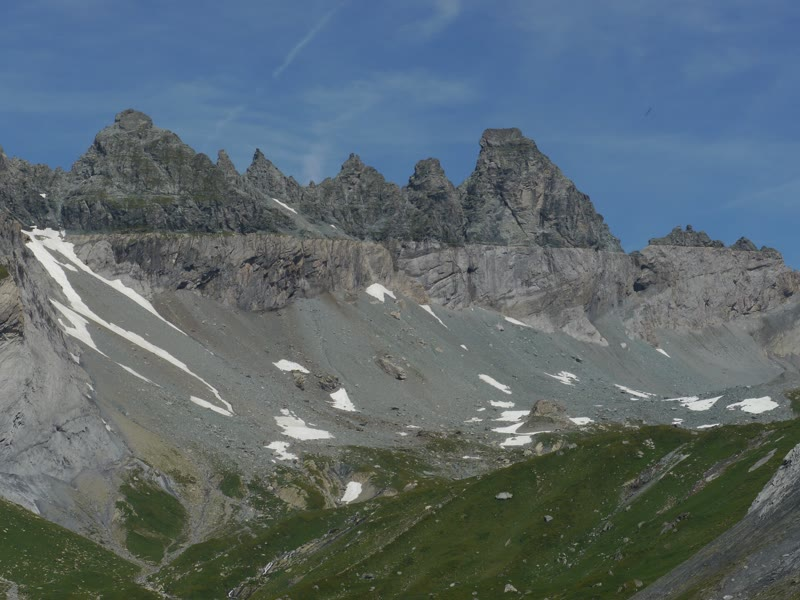
\includegraphics[width=0.5\linewidth]{images/book2/g12-heine-glarus-thrust.jpg}

{\small 瑞士东部阿尔卑斯山的格拉鲁斯\omterm{def:g12:mountain-building:thrust}{逆冲}断层。峰顶的深色岩层形成于二叠纪，
沉积于约 2.99 亿至 2.52 亿年前，
覆于颜色较浅、年代远为年轻的岩层之上；\omterm{def:g12:mountain-building:thrust}{逆冲}断层即二者之间的清晰界线。
\omterm{def:g11:fossil-fuel-geology:petroleum-system}{上覆岩层}已被推移约 40 至
\qty{50}{km}。照片：Christian Heine（CC~BY-SA~3.0）。}
\end{omfigure}
% ledger: photo:g12-glarus (Verrucano, Permian; displacement 40-50 km, Pfiffner 1985), ics:base.Permian, ics:base.Triassic

\subsection{测量缩短量}

\omterm{def:g12:mountain-building:fold}{褶皱}与\omterm{def:g12:mountain-building:thrust}{逆冲}断层都会使地壳
在受挤压的方向上缩短。

\begin{definition}[缩短量]\label{def:g12:mountain-building:shortening}
称一层岩层的\emph{缩短量}\index{缩短量}为其长度中已损失的比例：若原长为 $L_0$，
现跨度为 $L$，则
\[
  e = \frac{L_0 - L}{L_0}.
\]
\end{definition}

要测量它，需要知道原长 $L_0$。在许多\omterm{def:g12:mountain-building:fold}{褶皱}中，岩层
在弯曲时保持厚度不变，像弯折书本的书页那样相互滑动；
这样的岩层沿其长度方向并未被拉伸。
由此即可得到原长。
% ledger: tulane:fold-geometry (flexural folds keep their thickness)

\begin{proposition}[褶皱岩层的缩短量]\label{prop:g12:mountain-building:shortening}
若一层岩层发生\omterm{def:g12:mountain-building:fold}{褶皱}，且沿自身方向既未被拉伸也未被挤压，
则其原长 $L_0$ 等于沿\omterm{def:g12:mountain-building:fold}{褶皱}岩层量得的长度。
对于两翼为直线、倾角为 $\theta$ 的\omterm{def:g12:mountain-building:fold}{褶皱}，
\[
  e = 1 - \cos\theta .
\]
\end{proposition}

\begin{proof}
将岩层展开而不加拉伸，使其摊平，长度不变，
故 $L_0$ 即沿岩层的长度。在长为 $\ell$、倾角为 $\theta$ 的直线翼上，
所覆盖的水平距离
为 $\ell\cos\theta$（由直角三角形）。将所有翼相加，长为 $L_0$ 的岩层
跨度为 $L = L_0\cos\theta$，因此 $e = (L_0 - L_0\cos\theta)/L_0 =
1 - \cos\theta$。
\end{proof}

\begin{omfigure}
\begin{tikzpicture}
\begin{axis}[name=sine, x=2.0cm, y=2.0cm, axis lines=none,
  xmin=-0.05, xmax=2.25, ymin=-0.4, ymax=0.8, clip=false]
% computed in figdata/grade-12/fold_shortening.py (part sine: A/lambda = 0.25, e = 31.7 %)
\addplot[omLithSand!80!black, line width=1.6pt] table[x=x, y=y] {figdata/out/grade-12-fold_shortening-sine.dat};
\draw[omThm, line width=1.6pt] (axis cs:0,0.62) -- (axis cs:2.196,0.62);
\draw[black!60, |-|] (axis cs:0,-0.32) -- node[below, font=\scriptsize] {$L$（现今）} (axis cs:1.5,-0.32);
\node[anchor=south west, font=\scriptsize, omThm] at (axis cs:0,0.64) {$L_0$：展开后的同一岩层};
\end{axis}
\begin{axis}[omrecord, at={(sine.east)}, anchor=west, xshift=1.4cm, width=0.46\linewidth, height=4.6cm,
  xmin=0, xmax=80, ymin=0, ymax=85, xlabel={翼的倾角 $\theta$（\unit{\degree}）},
  ylabel={缩短量 $e$（\unit{\percent}）}, xtick={0,20,...,80}]
% computed in figdata/grade-12/fold_shortening.py (part dip: e = 1 - cos theta)
\addplot[omProp, line width=1pt] table[x=theta, y=e_pct] {figdata/out/grade-12-fold_shortening-dip.dat};
\addplot[only marks, mark=*, mark size=1.6pt, omThm] coordinates {(12,2.185) (30,13.397) (60,50)};
\node[anchor=south, font=\scriptsize, align=center] at (axis cs:12,6) {瓦尔登：\\\qty{2.2}{\percent}};
\node[anchor=west, font=\scriptsize] at (axis cs:32,10) {\qty{13}{\percent}};
\node[anchor=south east, font=\scriptsize] at (axis cs:60,51) {\qty{50}{\percent}};
\end{axis}
\end{tikzpicture}

{\small 左：\omterm{def:g12:mountain-building:fold}{褶皱}岩层跨度为 $L$；展开摊平、未被拉伸时，
其长为 $L_0$（此处\omterm{def:g12:mountain-building:fold}{褶皱}高度为其波长的四分之一，
且 $L$ 为 $L_0$ 的 \qty{68}{\percent}）。右：具有直线翼的\omterm{def:g12:mountain-building:fold}{褶皱}的
\omterm{def:g12:mountain-building:shortening}{缩短量} $1 - \cos\theta$，随
翼的倾角而变化。平缓的\omterm{def:g12:mountain-building:fold}{褶皱}使岩层缩短得很少。}
\end{omfigure}
% values: sine_025_e_pct 31.68 (L/L0 = 0.683); varden_e_pct 2.1852; chevron_30 13.397; chevron_60 50 (fold_shortening.py)

\begin{method}[在剖面上测量缩短量]\label{met:g12:mountain-building:shortening}
\begin{enumerate}
  \item 检查剖面是否按真实比例绘制。若其竖向比例被拉伸，
        则沿岩层的倾角和长度都会偏大：重新绘制，
        或先修正各倾角。
  \item 选取一条可在剖面上连续追踪的层界面；
        若被断层切断，则将两断开端恢复到断层移动前的位置，
        再连接起来。
  \item 沿岩层测量其长度 $L_0$：用细线沿其走向量取，
        或将若干短直线段相加。
  \item 测量其两端之间的水平距离 $L$。
  \item 计算 $e = (L_0 - L)/L_0$；若两翼为已知倾角的直线，
        则由 $e = 1 - \cos\theta$ 可直接求得。
\end{enumerate}
\end{method}

\begin{example}[瓦尔登褶皱]\label{ex:g12:mountain-building:varden}
瓦尔登\omterm{def:g12:mountain-building:fold}{褶皱}的两翼倾角为 \ang{12}，因此\omterm{def:g11:fossil-fuel-geology:reservoir}{盖层}的\omterm{def:g12:mountain-building:shortening}{缩短量}为
$e = 1 - \cos\ang{12} = 1 - 0.978 = 0.022$，约为 \qty{2.2}{\percent}：
该区域今日宽 \qty{10}{km}，\omterm{def:g12:mountain-building:fold}{褶皱}前的宽度为 $10/\cos\ang{12} \approx
\qty{10.22}{km}$。若按图中所画剖面 A--B 测量，
两翼看上去约 \ang{28} 陡，竖向比例被拉伸为 2.5 倍：
$\tan\theta$ 乘以 2.5，于是 $\arctan(2.5
\tan\ang{12}) \approx \ang{28}$。若照图面读取，
\omterm{def:g12:mountain-building:shortening}{缩短量}为 \qty{12}{\percent}，偏大五倍以上。
\end{example}
% values: varden_e_pct 2.1852, varden_L0_for_10km 10.223 (fold_shortening.py); arctan(2.5 x 0.2126) = 27.98 deg; 1 - cos 27.98 = 0.117

平缓\omterm{def:g12:mountain-building:fold}{褶皱}吸收的\omterm{def:g12:mountain-building:shortening}{缩短量}很少。一条紧密\omterm{def:g12:mountain-building:fold}{褶皱}带，
两翼倾角达 \ang{60}，缩短了一半；而一条几乎水平的\omterm{def:g12:mountain-building:thrust}{逆冲}断层，
若推送了一个 \qty{40}{km} 的\omterm{def:g12:mountain-building:nappe}{推覆体}，它吸收的\omterm{def:g12:mountain-building:shortening}{缩短量}为 \qty{40}{km}，
与一个很宽的平缓\omterm{def:g12:mountain-building:fold}{褶皱}带相当。

\section{增厚与隆升}

缩短并不会破坏岩石。一段地壳被挤压至其原宽度的一小部分，
其体积保持不变，因此必然增厚：若厚度为 $H_0$ 的地壳
沿造山带全长由宽度 $L_0$ 缩短为 $L$，
则其截面面积保持不变，即 $H L = H_0 L_0$，于是
\[
  H = H_0\,\frac{L_0}{L} = \frac{H_0}{1 - e}.
\]
一段厚 \qty{35}{km} 的地壳缩短 \qty{50}{\percent} 后，
厚度变为 \qty{70}{km}。随后由\omterm{def:g11:lithosphere-asthenosphere:isostasy}{地壳均衡}完成其余过程：较厚的地壳浮得更高，
其下的根部也更深（见\cref{prop:g11:lithosphere-asthenosphere:airy}）。
按艾里模型并采用回顾中的密度，厚度增加 $\Delta H$ 的地壳，
其高出的部分为 $\Delta H\,(\rho_m - \rho_c)/\rho_m = \Delta H
\times 550/3380$，约占增厚部分的六分之一；其余五分之六形成根部。
远离山脉处的地壳厚 \num{35} 至 \qty{40}{km}，
山脉之下则厚 50 至 \qty{70}{km}：山越高，
地壳越厚。
% ledger: tulane:roots, cm95:crust, data:prem

这就是珠穆朗玛峰峰顶海底石灰岩的由来：它们曾沉积于海底，
随印度向北\omterm{def:g11:fossil-fuel-geology:migration}{运移}，堆叠于喜马拉雅的\omterm{def:g12:mountain-building:thrust}{逆冲}岩片之中，
并随其下地壳增厚而被抬升，
隆起。这种地壳的竖直运动称为隆升。
% ledger: sakai05:summit, sakai05:stacking, tulane:roots (uplift), usgs:himalaya-collision

\section{两座山脉}

\subsection{喜马拉雅山脉}

喜马拉雅山脉沿印度与西藏的边界延伸 \qty{2900}{km}。
约 8000 万年前，印度位于亚洲以南约 \qty{6400}{km} 处，中间隔着一片海洋，
并以每年约 \qty{9}{cm} 的速度向北运动；它于 4000 万至 5000 万年前与亚洲相遇，
此后北进速度放缓。
板块重建较为详细地展示了这一历程：它综合多种证据，
其中包括热点的轨迹
（见\cref{ch:g11:plate-motions}），将板块逐步回溯到过去，
一步一步地推算。
% ledger: usgs:himalaya-collision, muller19:frame, muller22:frame

\begin{omfigure}
\begin{tikzpicture}
\begin{axis}[omrecord, omage, name=lat, width=0.5\linewidth, height=5.2cm,
  xmin=0, xmax=100, ymin=-45, ymax=35, xlabel={年龄 (\unit{Ma})}, ylabel={纬度 (\unit{\degree})},
  xtick={0,20,...,100}, ytick={-40,-20,...,40},
  legend style={font=\scriptsize, at={(0.98,0.03)}, anchor=south east, fill=white}]
% computed in figdata/grade-12/india_drift.py (part lat; GPlates Web Service, MULLER2022 and MULLER2019)
\fill[omThm!12] (axis cs:40,-45) rectangle (axis cs:50,35);
\addplot[omThm, line width=1.1pt] table[x=age, y=m22_india] {figdata/out/grade-12-india_drift-lat.dat};
\addplot[omThm, dashed, line width=0.8pt] table[x=age, y=m19_india] {figdata/out/grade-12-india_drift-lat.dat};
\addplot[omDef, line width=1.1pt] table[x=age, y=m22_lhasa] {figdata/out/grade-12-india_drift-lat.dat};
\addplot[black!50, line width=0.4pt, forget plot] coordinates {(0,0) (100,0)};
\legend{{印度中部（2022）}, {印度中部（2019）}, {拉萨（2022）}}
\end{axis}
\begin{axis}[omrecord, omage, at={(lat.east)}, anchor=west, xshift=1.9cm, width=0.42\linewidth, height=5.2cm,
  xmin=0, xmax=100, ymin=0, ymax=160, xlabel={年龄 (\unit{Ma})},
  ylabel={北向速度 (\unit{mm/\text{年}})}, xtick={0,20,...,100}]
% computed in figdata/grade-12/india_drift.py (part steps: 5-Myr steps)
\fill[omThm!12] (axis cs:40,0) rectangle (axis cs:50,160);
\addplot[omThm, line width=1pt] table[x=age, y=m22] {figdata/out/grade-12-india_drift-steps.dat};
\addplot[omThm, dashed, line width=0.7pt] table[x=age, y=m19] {figdata/out/grade-12-india_drift-steps.dat};
\end{axis}
\end{tikzpicture}

{\small 左图：印度中部某点（今日位于 \ang{78}~东经，
\ang{20}~北纬）及\omterm{def:g12:mountain-building:suture}{缝合带}以北的拉萨，在过去 1 亿年间的纬度变化，
取自两项已发表的板块重建（2022 年与 2019 年）。
右图：印度在每个 500 万年时段内的北向速度。阴影带
标出 4000 万至 5000 万年前的时段。数据来源：R.~D.~Müller 等人
（2019，2022），借助 GPlates Web Service 计算。}
\end{omfigure}
% ledger: data:b2-gws-india, muller22:frame, muller19:frame; values: speed_65_50 128.5, speed_40_0 40.06, fastest 145.8 (50-55 Ma) (india_drift.py)

两项重建结果相差在几度以内。6500 万至 5000 万年前，
印度以约每年 \qty{13}{cm} 的速度向北运动；5000 万至 4000 万年前，
其速度下降，而
自 4000 万年前至今，它以约每年 \qty{4}{cm} 的速度运动，不足前者的三分之一。
拉萨位于亚洲一侧，同样向北运动，
但速度慢得多。
% values: speed_65_50 128.5 mm/yr, speed_40_0 40.06 mm/yr, slowdown_ratio 0.312 (india_drift.py)

\begin{example}[印度的速度]\label{ex:g12:mountain-building:india}
在 2022 年的重建中，印度中部于 6000 万年前位于南纬 \ang{12.10}，
而在 5000 万年前位于南纬 \ang{0.68}。纬度一度对应的距离为
$2\pi R/360 = 2\pi \times \qty{6371}{km}/360 \approx \qty{111.2}{km}$。
印度在 1000 万年间向北移动了 $(12.10 - 0.68) \times 111.2 \approx \qty{1270}{km}$，
即每百万年 \qty{127}{km}，亦即 $\qty{127e6}{mm} /
\num{e6}\text{ 年} = \qty{127}{mm}$，约每年 \qty{13}{cm}。
\end{example}
% ledger: data:b2-gws-india, earth:Rmean; values: lat 60 Ma -12.0964, 50 Ma -0.6801 (india_drift-lat)

这种减速被视为碰撞的标志：抵达海沟的陆壳无法下沉，印度因此受阻。
首次接触的确切时间仍有争议，估计值
约在 6000 万至 5400 万年前之间，也有部分地质学家认为，
印度最先遇到的是一条火山岛链，直至
约 3400 万年前才真正抵达亚洲。印度至今仍未停止运动：当今板块的旋转极使其
以约每年 \qty{4.5}{cm} 的速度朝欧亚大陆推进，穿越喜马拉雅地区
（见\cref{ch:g11:plate-motions}），其挤压作用使亚洲的部分地区
向东推移。
% ledger: usgs:himalaya-collision, najman21:collision-age; values: today_in_eu_speed 44.99 mm/yr (india_drift.py, from nnr56:poles)

喜马拉雅以北的青藏高原平均海拔约 \qty{4600}{m}，
其下地壳厚约 \qty{70}{km}
（见\cref{ch:g11:lithosphere-asthenosphere}）。印度与西藏之间是
印度河–雅鲁藏布江\omterm{def:g12:mountain-building:suture}{缝合带}及其中的\omterm{def:g12:mountain-building:ophiolite}{蛇绿岩}；其南侧的喜马拉雅
主要由沉积于印度北缘的沉积物组成，随后经堆叠、\omterm{def:g12:mountain-building:fold}{褶皱}与断裂，
其中包括珠穆朗玛峰的峰顶石灰岩。
% ledger: karplus:tibet-moho, liu20:itsz, sakai05:stacking, sakai05:summit; Book 1: usgs:himalaya (Tibetan Plateau about 4600 m)

\subsection{阿尔卑斯山与整条山带}

阿尔卑斯山的历史与此相似，只是规模较小：它们隆起于非洲
与欧洲碰撞之处。其中同样含有\omterm{def:g12:mountain-building:ophiolite}{蛇绿岩}和巨大的\omterm{def:g12:mountain-building:thrust}{逆冲}构造：在
格拉鲁斯\omterm{def:g12:mountain-building:thrust}{逆冲}断层处，二叠纪岩层已被推覆到远为年轻的岩层之上。
阿尔卑斯山与喜马拉雅山属于同一条绵长的山带，
穿越伊朗的扎格罗斯山，非洲与印度在那里与欧亚\omterm{def:g12:mountain-building:collision}{大陆碰撞}。
% ledger: earle:collision, photo:g12-glarus

\begin{omfigure}
\begin{tikzpicture}
\begin{axis}[axis equal image, xmin=-12, xmax=105, ymin=18, ymax=52, width=\linewidth,
  tick label style={font=\scriptsize}, xtick={0,30,60,90}, ytick={20,30,40,50},
  xticklabel={$\pgfmathprintnumber{\tick}^\circ$}, yticklabel={$\pgfmathprintnumber{\tick}^\circ$},
  axis background/.style={fill=omSea}, legend columns=3,
  legend style={font=\scriptsize, at={(0.5,-0.12)}, anchor=north, /tikz/every even column/.append style={column sep=5pt}}]
\addplot[fill=omLithAlluv, draw=black!45, line width=0.2pt, forget plot] table {figdata/out/shared-geo-land.dat};
% computed in figdata/grade-12/alpine_belt.py; ledger: data:etopo1, data:usgs-comcat
\addplot[only marks, mark=square*, mark size=1.15pt, omLithSand!85!black] table[x=lon, y=lat] {figdata/out/grade-12-alpine_belt-high.dat};
\addplot[only marks, mark=square*, mark size=1.15pt, omThm!75!black] table[x=lon, y=lat] {figdata/out/grade-12-alpine_belt-higher.dat};
\addplot[only marks, mark=*, mark size=0.7pt, black] table[x=lon, y=lat] {figdata/out/grade-12-alpine_belt-quakes.dat};
\addplot[omDef, line width=0.9pt, forget plot] table {figdata/out/shared-geo-school-collision.dat};
\addplot[black!70, line width=0.5pt, forget plot] table {figdata/out/shared-geo-school-subduction.dat};
\legend{{高于 \qty{1500}{m}}, {高于 \qty{3500}{m}}, {地震，震级 6 或以上}}
\coordinate (alps) at (axis cs:9,48);
\coordinate (zagros) at (axis cs:46,23.5);
\coordinate (zagrosbelt) at (axis cs:50.5,31.5);
\coordinate (himal) at (axis cs:84,24);
\coordinate (tibet) at (axis cs:88,33);
\coordinate (arrA) at (axis cs:77,19.5);
\coordinate (arrB) at (axis cs:79.2,25);
\end{axis}
% labels drawn after the axis, so that no earthquake dot covers them
\node[font=\scriptsize, fill=white, inner sep=1pt, anchor=south] at (alps) {阿尔卑斯山};
\draw[black!60, line width=0.4pt] (zagros) -- (zagrosbelt);
\node[font=\scriptsize, fill=white, inner sep=1pt] at (zagros) {扎格罗斯山};
\node[font=\scriptsize, fill=white, inner sep=1pt, anchor=west] at (himal) {喜马拉雅山};
\node[font=\scriptsize, fill=white, inner sep=1pt] at (tibet) {青藏高原};
\draw[-{Stealth[length=2mm]}, line width=1pt, omProp] (arrA) -- (arrB);
\end{tikzpicture}

{\small 自大西洋至西藏的年轻山带：高地
（每个方格为 1 度网格），震级 6 或以上的浅源地震
（1976 年至 2025 年，震源深度浅于 \qty{70}{km}），以及
板块之间的碰撞型边界（蓝线）。箭头表示印度
向欧亚大陆的运动。数据来源：ETOPO1、USGS 地震目录、Bird（2003）的板块边界，
陆地数据来自 Natural Earth。}
\end{omfigure}
% ledger: data:etopo1, data:usgs-comcat, data:pb2002, data:ne-land; values: n_quakes 398 (alpine_belt.py)

高地与地震沿同一狭窄的带状区域分布。
碰撞尚未结束：地震表明，地壳仍在
沿整条山带破裂，山脉也仍在不断形成。

\section{练习}

\begin{exercise}[$\star$]\label{exo:g12:mountain-building:1}
将每个术语与其描述配对：\omterm{def:g12:mountain-building:fold}{背斜}、\omterm{def:g12:mountain-building:fold}{向斜}、\omterm{def:g12:mountain-building:thrust}{逆冲}、\omterm{def:g12:mountain-building:nappe}{推覆体}、
\omterm{def:g12:mountain-building:suture}{缝合带}、\omterm{def:g12:mountain-building:ophiolite}{蛇绿岩}。(a) 倾角较缓的\omterm{def:g12:mountain-building:thrust}{逆断层}；(b) 一块
出露于陆地上的洋底；(c) 两翼向轴部倾斜的\omterm{def:g12:mountain-building:fold}{褶皱}；
(d) 两个大陆曾相拼接之处；(e) 两翼背离轴部倾斜的\omterm{def:g12:mountain-building:fold}{褶皱}；
(f) 沿\omterm{def:g12:mountain-building:thrust}{逆冲}断层远距离搬运的大片岩席。
\end{exercise}

\begin{exercise}[$\star$]\label{exo:g12:mountain-building:2}
横穿一个山谷，西侧岩层向西倾斜 \ang{20}，
东侧岩层向东倾斜 \ang{20}。(1) 两者之间的\omterm{def:g12:mountain-building:fold}{褶皱}是
\omterm{def:g12:mountain-building:fold}{背斜}还是\omterm{def:g12:mountain-building:fold}{向斜}？(2) 经侵蚀后，
沿其轴部出露的是最老还是最新的岩层？(3) 山谷下方是否必然为\omterm{def:g12:mountain-building:fold}{向斜}？
\end{exercise}

\begin{exercise}[$\star$]\label{exo:g12:mountain-building:3}
某岩层\omterm{def:g12:mountain-building:fold}{褶皱}，两翼为直线，倾角 \ang{30}。(1) 计算其
\omterm{def:g12:mountain-building:shortening}{缩短量}。(2) 现今跨度为 \qty{6.0}{km}，其原始长度为多少？
\end{exercise}

\begin{exercise}[$\star$]\label{exo:g12:mountain-building:4}
(1) 沿某断层，断层面上盘向下移动。它是
\omterm{def:g11:ocean-ridges:normal-fault}{正断层}还是\omterm{def:g12:mountain-building:thrust}{逆断层}？地壳是受拉伸还是受挤压？
(2) 倾角为 \ang{25} 的\omterm{def:g12:mountain-building:thrust}{逆断层}是否属于\omterm{def:g12:mountain-building:thrust}{逆冲}断层？
\end{exercise}

\begin{exercise}[$\star$]\label{exo:g12:mountain-building:5}
(1) 将\omterm{def:g12:mountain-building:ophiolite}{蛇绿岩}中的以下岩石按自上而下排序：\omterm{def:g11:ocean-ridges:gabbro}{辉长岩}、
海相沉积物、\omterm{def:g11:ocean-ridges:peridotite}{橄榄岩}、枕状玄武岩、席状\omterm{def:g11:igneous-rocks:intrusion}{岩墙}。(2) 为何
枕状玄武岩表明该岩石形成于水下？(3) 为何
\omterm{def:g12:mountain-building:ophiolite}{蛇绿岩}沿\omterm{def:g12:mountain-building:suture}{缝合带}分布？
\end{exercise}

\begin{exercise}[$\star\star$]\label{exo:g12:mountain-building:6}
在真实比例的剖面图上，一条砂岩边界被追踪，穿过四段
直线段，长度分别为 \qty{2.1}{km}、\qty{1.8}{km}、\qty{2.4}{km} 和
\qty{1.6}{km}；其两端相距 \qty{6.0}{km}。(1) 计算
\omterm{def:g12:mountain-building:shortening}{缩短量}。(2) 若四段的倾角都相同，该倾角为多少？
\end{exercise}

\begin{exercise}[$\star\star$]\label{exo:g12:mountain-building:7}
倾角为 \ang{10} 的\omterm{def:g12:mountain-building:thrust}{逆冲}断层，其上盘沿
断层面移动了 \qty{45}{km}。(1) 其水平方向移动了多少？(2) 其
上升高度为多少？(3) 翼部倾角为 \ang{12} 的\omterm{def:g12:mountain-building:fold}{褶皱}带需要多宽，才能
吸收相同的水平\omterm{def:g12:mountain-building:shortening}{缩短量}？
\end{exercise}

\begin{exercise}[$\star\star$]\label{exo:g12:mountain-building:8}
沿麦克康内尔\omterm{def:g12:mountain-building:thrust}{逆冲}断层，约 5 亿年的石灰岩覆盖在
约 7500 万年的泥岩之上。(1) 若地质学家忽略了断层，哪一条相对定年
原理会误导他？(2) 上部岩石
比下部岩石老多少？(3) \omterm{def:g12:mountain-building:thrust}{逆冲}岩席厚约 \qty{800}{m}，移动了
\qty{40}{km}：这是其自身厚度的多少倍？
\end{exercise}

\begin{exercise}[$\star\star$]\label{exo:g12:mountain-building:9}
2022 年重建模型中，印度中部在 8000 万年前
位于南纬 \ang{30.23}~，并在 6600 万年前位于南纬 \ang{19.38}~。(1) 该地
向北移动了多远？(2) 平均速度为多少，单位为 \unit{cm}/年？(3) 与
美国地质调查局的概括结论相比较，约为每世纪 \qty{9}{m}。
\end{exercise}

\begin{exercise}[$\star\star$]\label{exo:g12:mountain-building:10}
一段厚 \qty{35}{km} 的地壳在
整个造山带上缩短了 \qty{40}{\percent}。(1) 其厚度变为多少？(2) 取 $\rho_c =
\qty{2830}{kg/m^3}$，$\rho_m = \qty{3380}{kg/m^3}$，该地壳会高出多少，
其额外的根部深入多深？
\end{exercise}

\begin{exercise}[$\star\star$]\label{exo:g12:mountain-building:11}
在竖直方向被放大 3 倍的剖面图上，某翼部看起来
倾斜 \ang{40}。(1) 其真实倾角为多少？(2) 分别依据真实倾角和
图上读出的倾角，计算\omterm{def:g12:mountain-building:shortening}{缩短量}。(3) 用于测量\omterm{def:g12:mountain-building:shortening}{缩短量}的剖面图
为什么必须按真实比例绘制？
\end{exercise}

\begin{exercise}[$\star\star\star$]\label{exo:g12:mountain-building:12}
本章所绘的圆顶状\omterm{def:g12:mountain-building:fold}{褶皱}，其高度约为
波长的四分之一，\omterm{def:g12:mountain-building:shortening}{缩短量}为 \qty{31.7}{\percent}；其最陡倾角约为
\ang{57.5}。(1) 一层以此方式\omterm{def:g12:mountain-building:fold}{褶皱}的岩层横跨 \qty{10}{km}，
它原来有多长？(2) 计算翼部为直线、倾角为
\ang{57.5} 的\omterm{def:g12:mountain-building:fold}{褶皱}的\omterm{def:g12:mountain-building:shortening}{缩短量}。(3) 解释为什么在最陡倾角相同时，
直线翼\omterm{def:g12:mountain-building:fold}{褶皱}的\omterm{def:g12:mountain-building:shortening}{缩短量}更大。
\end{exercise}

\begin{exercise}[$\star\star\star$]\label{exo:g12:mountain-building:13}
在喜马拉雅山以北，位于东经 \ang{85}~，北纬 \ang{28}~，由转动极给出印度
相对于欧亚大陆的速度为：向东 \qty{16.6}{mm/\text{年}}，
向北 \qty{41.8}{mm/\text{年}}。在过去 500 万年间，2022
年重建模型给出印度中部的向北速度，比拉萨的向北速度快
\qty{23.5}{mm/\text{年}}。(1) 求印度相对于
欧亚大陆的速度。(2) 假设北向分量可以比较，
则拉萨以北地区每百万年仍需吸收的
南北向\omterm{def:g12:mountain-building:shortening}{缩短量}为多少？(3) 本章中哪里有该地区正在变形的标志？
\end{exercise}

\begin{exercise}[$\star\star\star$]\label{exo:g12:mountain-building:14}
在阿尔卑斯山，一个\omterm{def:g12:mountain-building:nappe}{推覆体}沿一条倾角
接近零的\omterm{def:g12:mountain-building:thrust}{逆冲}断层被推送了 \qty{45}{km}。(1) 该\omterm{def:g12:mountain-building:thrust}{逆冲}断层吸收了多大的\omterm{def:g12:mountain-building:shortening}{缩短量}？(2) 要吸收相同的\omterm{def:g12:mountain-building:shortening}{缩短量}，
像瓦尔登丘陵（翼部倾角
\ang{12}）那样的\omterm{def:g12:mountain-building:fold}{褶皱}\omterm{def:g11:fossil-fuel-geology:reservoir}{盖层}，在\omterm{def:g12:mountain-building:fold}{褶皱}前的宽度需为多少？(3) 这说明
山脉如何吸收大量的汇聚？
\end{exercise}

\begin{exercise}[$\star\star\star$]\label{exo:g12:mountain-building:15}
珠穆朗玛峰顶部的石灰岩沉积于海底，至少
位于海平面之下一点，如今其高度为 \qty{8848.86}{m}。(1) 假设
碰撞始于 5000 万年前，则最小平均隆升速率为多少，
单位为 \unit{mm}/年？(2) 将其与印度自
4000 万年前以来的速度相比较，后者约为 \qty{40}{mm}/年。(3) 为什么岩石的
隆升量很可能大于其现今高度？
\end{exercise}

\begin{problem}[{周末问题——印度之旅}]
\label{pb:g12:mountain-building:1}
% ledger: data:b2-gws-india, earth:Rmean, usgs:himalaya-collision, tulane:roots, cm95:crust, data:prem, karplus:tibet-moho; Book 1: usgs:himalaya (4600 m)
% values: india_drift-lat (MULLER2022, rounded to 0.01 deg); north_since_66_km 4378.7; converge_since_50 1354; gap_0 1073
下表给出 2022 年板块重建模型中印度中部某点及拉萨的纬度，
拉萨位于\omterm{def:g12:mountain-building:suture}{缝合带}以北（负值表示南纬）。
取纬度一度为 \qty{111.2}{km}，并取 \qty{1}{km} 每百万年
相当于 \qty{1}{mm} 每年。

\begin{center}
\small
\begin{tabular}{|l|c|c|c|c|c|c|c|c|c|}
\hline
年龄（\unit{Ma}） & 80 & 66 & 60 & 55 & 50 & 45 & 40 & 20 & 0 \\ \hline
印度（\unit{\degree}） & $-30.23$ & $-19.38$ & $-12.10$ & $-7.24$ & $-0.68$ & 3.30 & 5.59 & 13.40 & 20.00 \\ \hline
拉萨（\unit{\degree}） & & 19.48 & & & 21.15 & & & & 29.65 \\ \hline
\end{tabular}
\end{center}

\medskip
\noindent\textbf{第一部分——纬度与速度。}
\begin{enumerate}
  \item 检验一度为 \qty{111.2}{km} 的取值，取 $R =
        \qty{6371}{km}$。
  \item 印度中部何时越过赤道？
  \item 印度从 6600 万年前到 5000 万年前向北移动了多远？
  \item 平均速度为多少？
  \item 计算从 6600 万年前到 4000 万年前各阶段的速度（6600
        至 6000 万年前，6000 至 5500 万年前，依此类推）。哪一阶段最快？
\end{enumerate}

\medskip
\noindent\textbf{第二部分——减速。}
\begin{enumerate}[resume]
  \item 计算印度从 4000 万年前到现今的平均速度。
  \item 该速度是其从 6600 万年前到 5000 万年前速度的几分之几？
  \item 表中哪两个时间点之间速度下降最多？
  \item 为什么碰撞会使板块减速？
  \item 印度从 5000 万年前到现今向北移动了多远？
\end{enumerate}

\medskip
\noindent\textbf{第三部分——吸收的汇聚。}
\begin{enumerate}[resume]
  \item 拉萨从 5000 万年前到现今向北移动了多远？
  \item 自 5000 万年前以来，印度中部与拉萨之间的
        南北距离缩短了多少？
  \item 该距离现今为多少，5000 万年前又是多少？
  \item 假设这一汇聚全部由两点之间的地壳缩短所吸收，
        求\omterm{def:g12:mountain-building:shortening}{缩短量} $e$。
  \item 说出吸收这种缩短的两类构造。
\end{enumerate}

\medskip
\noindent\textbf{第四部分——地壳增厚。}
\begin{enumerate}[resume]
  \item 若该地壳 5000 万年前厚 \qty{35}{km}，
        保持其截面不变，现今会有多厚？
  \item 取 $\rho_c = \qty{2830}{kg/m^3}$ 与 $\rho_m = \qty{3380}{kg/m^3}$，
        它会比原来的水平高出多少？
  \item 青藏高原约高 \qty{4600}{m}，其下地壳
        厚约 \qty{70}{km}。按艾里模型，
        高 \qty{4600}{m} 处的地壳厚度应为多少？
  \item 给出一个理由，说明第 16 题中的简单模型为何高估了
        增厚。
  \item 将第 3 题与第 10 题中的距离相加，印度
        自白垩纪末（6600 万年前）以来
        向北移动了多远？
\end{enumerate}
\end{problem}
